\documentclass[letterpaper, 9pt, conference]{ieeeconf}

\usepackage{amssymb}\usepackage{amsmath}\usepackage{amsfonts}
\usepackage[mathcal, mathscr]{eucal}
\usepackage{graphicx}
\usepackage{epstopdf}
\newcommand{\vect}{\boldsymbol}
\newcommand{\matr}{\boldsymbol}
\newcommand{\diag}{\textrm{diag}}
\usepackage{algorithm}
\usepackage{algorithmic}

\IEEEoverridecommandlockouts       % This command is only
                                                          % needed if you want to
                                                          % use the \thanks command
\overrideIEEEmargins
% See the \addtolength command later in the file to balance the column lengths
% on the last page of the document

% The following packages can be found on http:\\www.ctan.org
%\usepackage{graphics} % for pdf, bitmapped graphics files
%\usepackage{epsfig} % for postscript graphics files
%\usepackage{mathptmx} % assumes new font selection scheme installed
%\usepackage{times} % assumes new font selection scheme installed
%\usepackage{amsmath} % assumes amsmath package installed
%\usepackage{amssymb}  % assumes amsmath package installed

\title{\LARGE \bf
Recurrence network analysis of multiple local field potential bands from the orofacial portion of primary motor cortex. 
}


% PIN:  26810 (ZC),
% 42117 (KT), 17447 (NGH)
% 67619  (Narayan) 
% 11131 (Jari) 
% CFR 58190 
% Session code v41rc
\author{Narayan Puthanmadam Subramaniyam$^{1}$, {\em Student Member, IEEE}, Jari Hyttinen$^{1}$, {\em Senior Member, IEEE}, \\
Nicholas G. Hatsopoulos$^{2,3}$, Callum F. Ross$^{2}$, and 
Kazutaka Takahashi$^{2}$, {\em Senior Member, IEEE} \\
\thanks{$^{1}$N.P.S. and J.H. are with Department of Elecronics and Communications Engineering, Tampere University o Technology. 
(Email: \{narayan.ps, jari.hyttinen\}@tut.fi.) This work is financially supported by International Doctoral Programme in Biomedical Engineering and Medical Physics (iBioMEP) – Academy of Finland, Decision No. 141171.}
\thanks{$^{2}$N.G.H. C.F.R. and K.T. are with the Department of Organismal Biology and Anatomy, University of Chicago, IL 60637, USA (e-mail: \{nicho, rossc, kazutaka\}@uchicago.edu). 
 (Email: kazutaka@uchicago.edu). This work was supported by NIH R01 DE023816
and R01 NS04853.
}
}

\begin{document}



\maketitle
\thispagestyle{empty}
\pagestyle{empty}


\begin{abstract}
Local field potentials (LFPs), which have been considered as aggregate signals that reflect activities of a large number of neurons in the cerebral cortex, have been observed to mediate gross functional activities of a relatively small volume of the brain tissues. Historically there have been several frequency bands observed and defined across various brain areas. However, detailed analysis, either spectral analysis or any dynamical analysis of LFPs particularly in the orofacial part of the primary motor cortex (MIo) has not been done before. Here, we recorded LFPs from MIo using an array electrode from a non-human primate during feeding behavior. Then we performed spectral analysis to identify power spectrum during the whole feeding sequences and to characterize temporal evolution of spetrum around the time of swallow cycles. The spectrogram over the $\beta$ range showed dynamica change in its power around the swallow cycle onsets. We then characterized dynamical behaviors of LFPs over multiple bands, $\alpha$, $\beta$, low $\gamma$, and high $\gamma$ using two measures from  the recurrence network (RN) method, network transitivity, $T$ and average path length $L$. Temporal profile of $T$ in $\alpha$ and $\beta$ indicated that there was a sudden change in the dynamical properties around the swallow cycle onsets, while temporal profile of $L$ indicated that a range of $-200$ to -$150$ ms and $200$ms to the swallow cycle onsets exhibited large changes both in $\alpha$ and $\beta$ ranges. Therefore, to further understand the involvement of cortical oscillation to behavior, particularly swallowing, the combination of various dynamical methods such as RN method would be essential. 

\end{abstract}

\begin{keywords}
Local field potentials, event evoked potentials, recurrence network, temporal dynamics, motor cortex
\end{keywords}



\section{Introduction}
Cortical rhythms have been studied since early descriptions of oscillations in sensorimotor cortex by Jasper and Penfield \cite{jasper1949}. 
Although our understanding of underlying circuitry for different bands of oscillations has increased over the years \cite{Womelsdorf2014}, we still know little about inherent dynamics of each of oscillation bands and their relation to behaviors. In particular, local field potentials (LFPs) and electroencephalograms (EEG) in the $\beta$ frequency range (15-30 Hz) are ubiquitous in the motor cortex of mammals including monkeys and humans across the primary motor cortex (MI). The dynamics of the $\beta$ oscillation has been grossly characterized, based on a temporal profile of the amplitude of the oscillations, such as event related synchronization (ERS) and event related desynchronization (ERD) \cite{neuper2001, Jurkiewicz20061281}, and phase locking to the instruction cues \cite{jake2011}. However, the dynamical properties of $\beta$ oscillations have not been well characterized. Recently, it has been reported that phase of $\beta$ oscillations propagated as plane waves along the rostrocaudal axis of the arm portion of MI during motor preparation and execution for upper arm movement, and are believed to subserve cortical information transfer \cite{doug2006betawave}. 

However, even in the same MI, the spectral properties of LFPs in the orofacial portion of MI have not been well characterized. Teismann's group showed \cite{Teismann2009} that prior to volitional swallowing, there is some dynamical behavior in $\beta$ range based on MEG recording. Furthermore, our recent preliminary study showed \cite{Takahashi2012a} that functional connection topology of spiking neurons recorded from the orofacial part of MI is drastically different between during rhythmic chewing cycles and transition from rhythmic chew to swallow cycles.  Thus we speculate that there should be some signature of change in $\beta$ oscillation around the beginning of swallow cycles. 

The dynamics of neural activities in general can be considered as nonlinear, mainly arising from the threshold and saturation phenomena \cite{andrzejak2001indications}. It has been recently shown that methods based on recurrence plots, particularly recurrence networks (RN) can be used to study the structural complexity of the EEG signals \cite{subramaniyam2014characterization, subramaniyam2013analysis}. One particular advantage of  RN based analysis is that it can be applied to short segments of data, since the network properties like the network transitivity $T$ \cite{boccaletti2006complex}, which is related to the clustering property of a network \cite{barrat2000properties} or average path length $L$ can still be reliably estimated. The topological characterization of the RN using such network properties can provide insights into the complexity of the dynamics associated with the time series \cite{donner2010recurrence}. 

Therefore, we first used spectral methods to identify any particular power concentrated on certain bands and temporal power variations. Then we used RN method to characterize inherent dynamics of four bands of LFPs, up to $\alpha$ (1- 10 Hz), $\beta$ (10-30 Hz), low $\gamma$ (30-80 Hz), and high $\gamma$ (80-200 Hz) using T and L around the time of swallow cycle onsets. 

%They represent the summed activity of multiple postsynaptic potentials near the recording electrode site. however, little is %known about the relationship between the wave propagation of cortical oscillations and the information flow
%among individual neurons across the motor cortex. Recently, directed
%information between pairs of neurons was studied using multiple
%spike trains in the MI of a monkey \cite{ref:Chris2011}, but they
%considered only pairwise directed information and did not analyze
%how the network might change in relationship to the stimulus.



%Less than alpha = 1-10 Hz 
%Beta = 10-30 Hz 
%Low gamma = 30:80 Hz 
%High gamma = 80:200 Hz 


\section{Method}
\label{sec:method}

\subsection{Behavior task and data collection}

All of the surgical and behavior procedures were approved by the University of Chicago IACUC and conform to the principles outlined in the Guide for the Care and Use of Laboratory Animals (NIH publication no 86-23, revised 1985). One female macaque monkey was trained to feed with her right hand while restrained in a primate chair. Her head was restrained with a halo coupled to the cranium through chronically implanted headposts. At least one month prior to data recording, three 0.5 mm diameter tantalum balls (RSA Biomedical, http://www.umrsa.com/) were implanted by hypodermic needle into the anterior, middle, and posterior regions of the tongue at midline, under isoflurane anesthesia. Post-surgery, the monkey was trained to perform a manual feeding task and eat various types of foods in preparation for videofluoroscopy (VF). While the monkey self-fed various foods, two-dimensional lateral view VF recordings of jaw and tongue movements were acquired at a frame rate of 100 Hz using an OEC 9600 C-arm fluoroscope retrofitted with a  Redlake  Motion  Pro  500  video  camera (Redlake MASD LLC, San Diego, CA, USA)  \cite{Callum2010a}. Detailed methods of collecting jaw kinematic data are described elsewhere  \cite{Reed2011,pepe2011}. Three dimensional jaw kinematic data were collected in the coordinate system of the cranium using an infrared light video-based motion analysis system (Vicon Motion Tracking System with 10 MX40 cameras with sampling rate of 250 Hz) which tracked reflective markers coupled to the mandible and cranium using bone screws. The marker coordinates were bi-directionally lowpass filtered with a 4th order Butterworth filter with 15 Hz cutoff frequency. Using movements of the mandibular marker, jaw movement cycles were defined by two consecutive maximum gapes (i.e., maximum open). The cycles in each feeding sequence were then assigned into five different cycle types: ingestion, manipulation, stage-1 transport, rhythmic chew and swallow \cite{Thexton1980} by checking the behavior with VF data. In this study, we focused on time windows $\pm 400$ ms around the beginning of swallow cycles. 


%transitions between two consecutive rhythmic chew cycles (Chew Transitions) and between rhythmic chewing and swallow cycles (Swallow Transitions). 94.4\% of chew cycle durations were shorter than 600 ms, with the mode and mean being approximately 300 ms. Thus 300 ms was used to represent a canonical duration of one chew cycle for the rest of the study.

We recorded local field potentials from a chronically implanted 100-electrode Utah microelectrode array (1.5 mm in length, 10 x 10 grid, 400 $\mu m$ interelectrode spacing, Blackrock Microsystems, Utah, USA,) in the orofacial area of primary motor cortex (MIo) on the left side of the monkey. LFPs from up to 96 channels were recorded at 1 kHz. The LFP data for each channel were filtered over $\alpha$ (3-10 Hz), $\beta$ (10-30 Hz), low $\gamma$ (30-80 Hz), and high $\gamma$ (80-200 Hz) respectively first, then were chunked into [-600, 599] ms centered on the maximum gape (or the beginning) of swallow cycles (74 events), then a sliding window of $400$ ms with a 1 ms increment was used to perform RN analysis over [-400,400] ms centered on the beginning of swallow cycles. 

\section{Recurrence Network Analysis}

Recurrences are a fundamental property of many dynamical processes and the method of recurrence plots (RPs) can be used to visualize recurrences in the phase space \cite{marwan2007recurrence}. Given a scalar time series $y(t) = \left\lbrace y_1,y_2,\cdots,y_N\right\rbrace $, one can reconstruct an $m$-dimensional phase space vector $\mathbf{y}_i = \left(y_i,y_{i+\tau},\cdots,y_{i+(m-1)\tau} \right) $ by choosing a suitable embedding dimension $m$ and lag $\tau$ \cite{kantz2004nonlinear}. A recurrence matrix can be given as

\begin{equation}
R_\varepsilon(i,j) = \Theta(\varepsilon - ||\mathbf{y}_i - \mathbf{y}_j),
\label{eq_1}
\end{equation}

where $\mathbf{y}_i$ and $\mathbf{y}_j$ are state vectors at time $t=t_i$ and $t_j$ respectively, $\Theta$ is the Heaviside function, $||\cdot||$ is the distance norm (manhattan or euclidean or maximum) and $\varepsilon$ is the recurrence threshold, which is basically the phase space distance. The recurrence matrix $\mathbf{R}_\varepsilon$ can be further reinterpreted as an adjacency matrix of a complex network using the following transformation \cite{donner2010recurrence,marwan2009complex}
\begin{equation}
A_\varepsilon(i,j) = R_\varepsilon(i,j) - \delta(i,j),
\label{eq_2}
\end{equation}
where $\delta(i,j)$ is the Kronecker delta to make the elements along the diagonal of the adjacency matrix $\mathbf{A}$ zero. The adjacency matrix $\mathbf{A}_\varepsilon$ represents a complex network known as the $\varepsilon$-recurrence network (RN). Also, the adjacency matrix $\mathbf{A}_\varepsilon$ preserves the symmetric properties of the recurrence matrix $\mathbf{R}_\varepsilon$ and thus the $\varepsilon$-recurrence network represents a simple graph \cite{donner2015complex}. Using graph theoretical measures, one can now characterize the structural properties of the underlying dynamical system represented by the univariate time series $y(t)$. The toolbox of complex network theory offers a repository of large measures. In this work, we look at two global measures, the network transitivity $T$ \cite{boccaletti2006complex}, which is related to the clustering property of a network \cite{barrat2000properties} and is given as,
 
\begin{equation}
T = \frac{\sum_{i,j,k = 1}^{N}A(i,j)A(j,k)A(k,i)}{\sum_{i,j,k = 1}^{N}A(i,j)A(k,i)},
\label{eq_3}
\end{equation}

and the average path length $L$ \cite{boccaletti2006complex} given as,

\begin{equation}
L =\frac{1}{N(N-1)}\sum_{ i\neq j} d(i,j),
\label{eq_4}
\end{equation}

where $d(i,j)$ is the geodesic distance between two vertices in a network and $N$ is the number of vertices. The network transitivity for a RN characterizes the global dimensionality of a system \cite{donner2011geometry}. Dynamical systems exhibiting periodic dynamics display high values for $T$ and $L$ compared to systems exhibiting chaotic dynamics. Thus, these measures give an insight into the regularity of the underlying dynamics. 

By dividing a time series into small windows, moving window recurrence network analysis can be performed to obtain a time-varying profile of these network measures. Using such an approach, one can identify dynamical transitions in a time series. Particularly, measures like $T$ and $L$ are sensitive to dynamical transitions in a complex system as demonstrated by their application to paleoclimate \cite{donner2011recurrence} and biogeoscience data \cite{lange2015recurrence} 


\section{Results}
\label{sec:results}
\subsection{Spectral profiles of LFPs}
\begin{figure}[ht!]
\begin{minipage}{20pc}
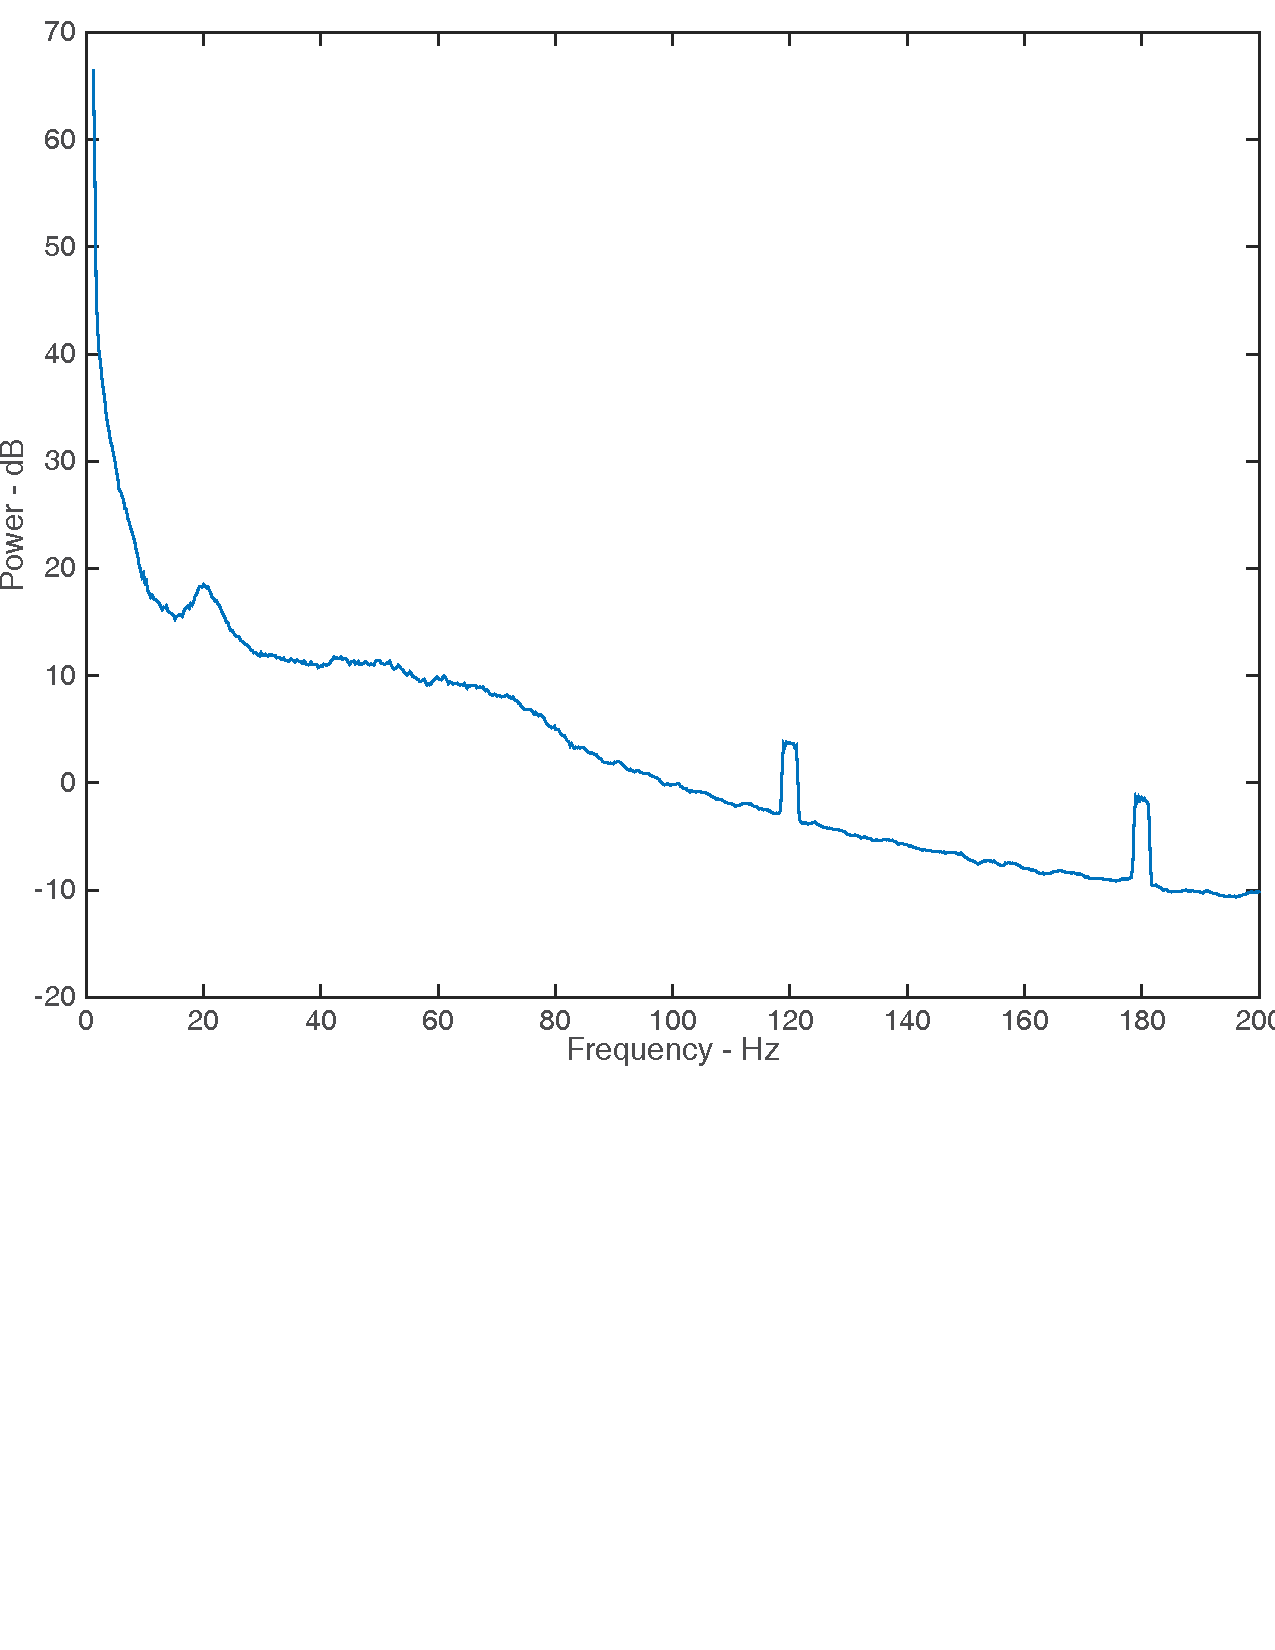
\includegraphics[width=20pc]{PSD_v1.pdf}
 \vspace{-1.5in}
\caption{\label{fig:psd}Averaged power spectrum of LFP computed over all channels recorded by MIo array. There is a clear peak around 20Hz in this subject over $\beta$ range and a small and wide peak in a low $\gamma$ range.There is line-noise at integer multiples of 60Hz and only 60Hz noise was removed by a notch filter.}
\end{minipage}\hspace{2pc}
\end{figure}

First, Fig. \ref{fig:psd} shows a power spectrum of LFPs computed over all feeding sequences across all channels. The multi-taper method from Chronux (http://chronux.org/) \cite{Mitra2008} was used and the parameters used were: $[TW, K]=[3, 5]$, where $TK$ denoted the time-bandwidth product and $K$ being the number of tapers. There were a distinct peak around 18-19 Hz over the $\beta$ oscillation and a small peak around $40$Hz over the low $\gamma$ range. $60$Hz line noise was notched out, but $120$Hz and $180$Hz noises were still present for Fig. \ref{fig:psd}. 

\begin{figure}[ht!]
\begin{minipage}{20pc}
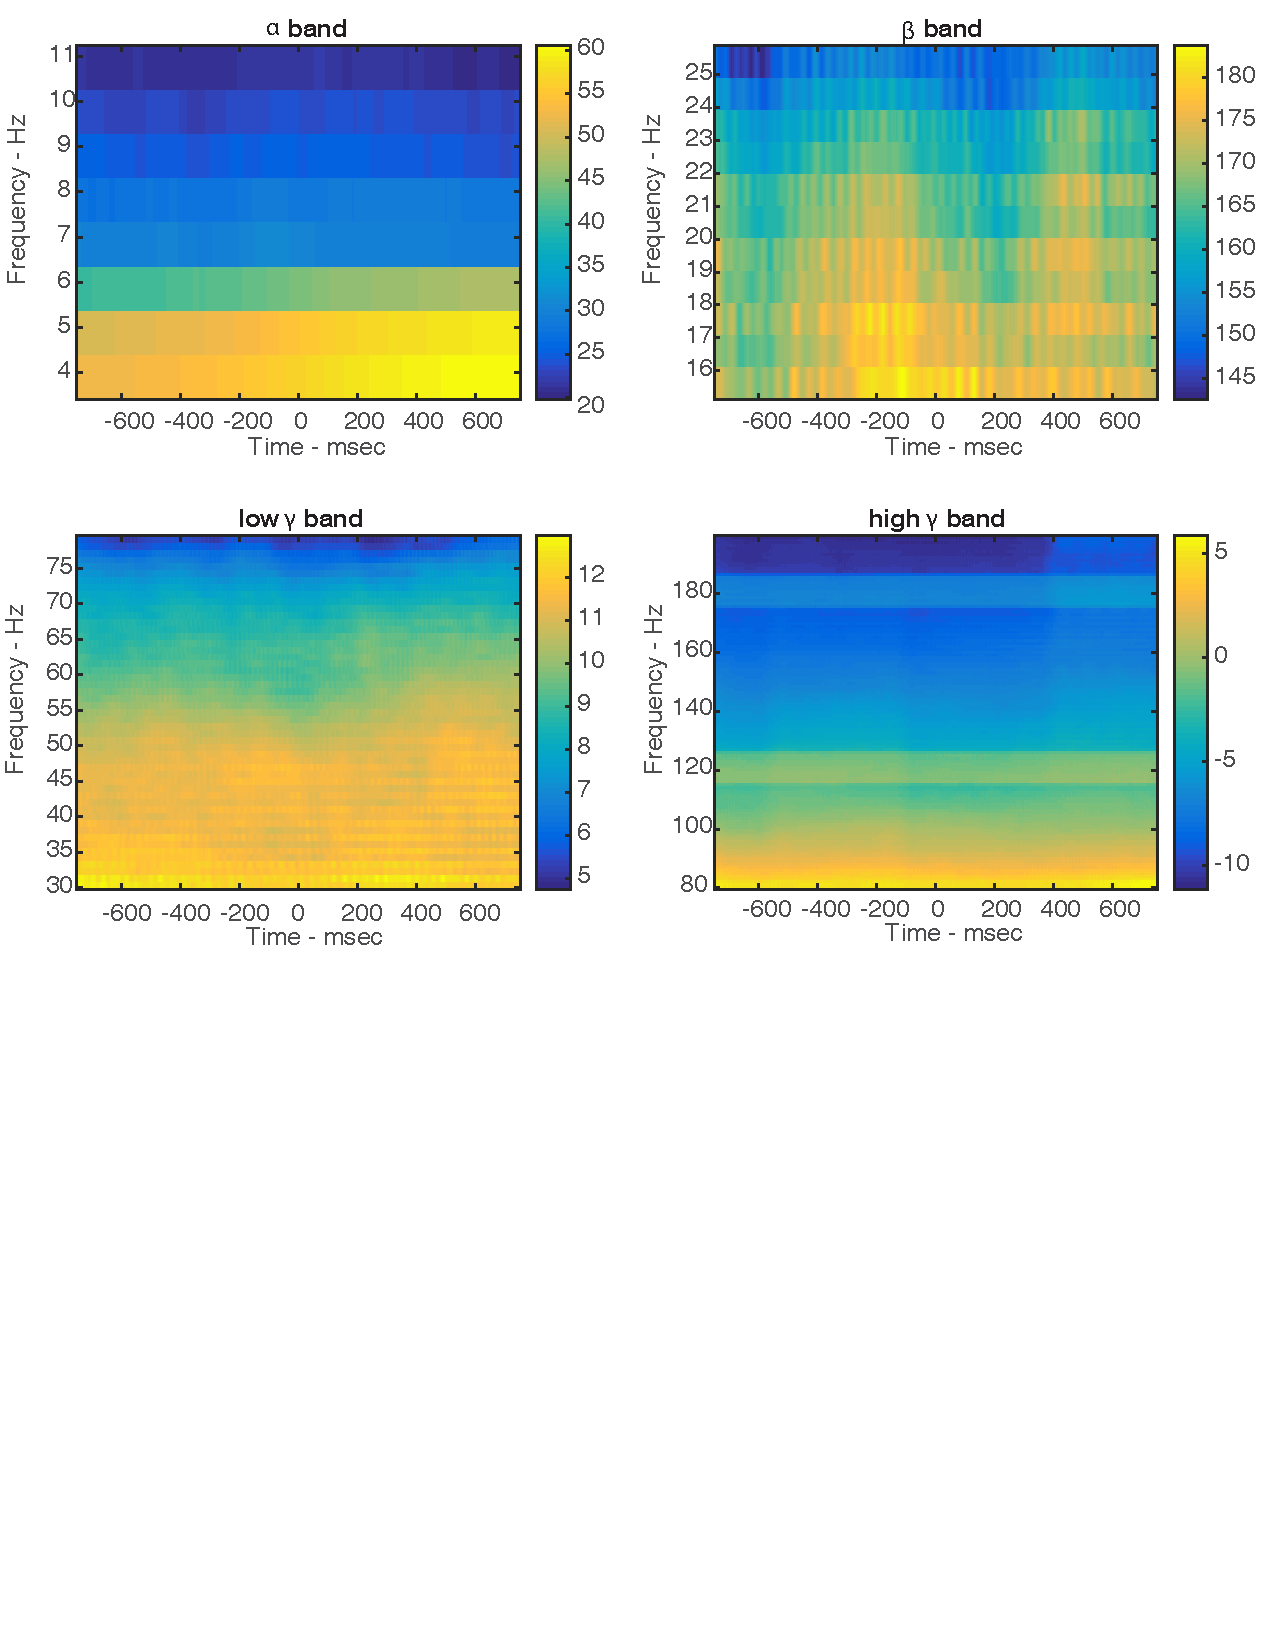
\includegraphics[scale=0.4]{spectrgram.pdf}
 \vspace{-2in}
\caption{\label{fig:psg} Spectrograms of 4 speficied bands of  LFP, $\alpha$, $\beta$, low $\gamma$ and high $\gamma$ ranges.}
\end{minipage}\hspace{2pc}
\end{figure}

Fig. \ref{fig:psg} showed a set of spectrograms of LFPs computed for $4$ bands over $[-700, 700]$ ms of all swallow cycle onsets. The parameters used for the multi-taper method were the same as above and a moving window of 500 ms with a 1 ms increment was used. There was a power increase in $\delta$-$\theta$ boundry 200-300 ms after swallow cycle onset. The $\beta$ range showed dynamical behavior starting with low power and peaks about $-200$ ms and kept attenuating and a weak increase again after $200$ ms from the onset. Neither low or high $\gamma$ ranges show significant modulations around the swallow cycle onsets.  


\subsection{Temporal profiles of  Network transitivity $T$  and Average path length $L$ across different bands}
The mean network transitivity $T$  for evoked responses across all channel for the four different frequency bands were shown in Fig. \ref{fig:GC_low}. The $\alpha$ and $\beta$ bands showed somewhat similar temporal profiles where sharp drops of $T$ around or slightly before $0$ ms and rebounding were observed. While the low $\gamma$ band somewhat monotonically decreased its $T$ valuesm the high $\gamma$ band exhibited a brief decrease around $200$ ms. 

\begin{figure}[ht!]
\begin{center}
                             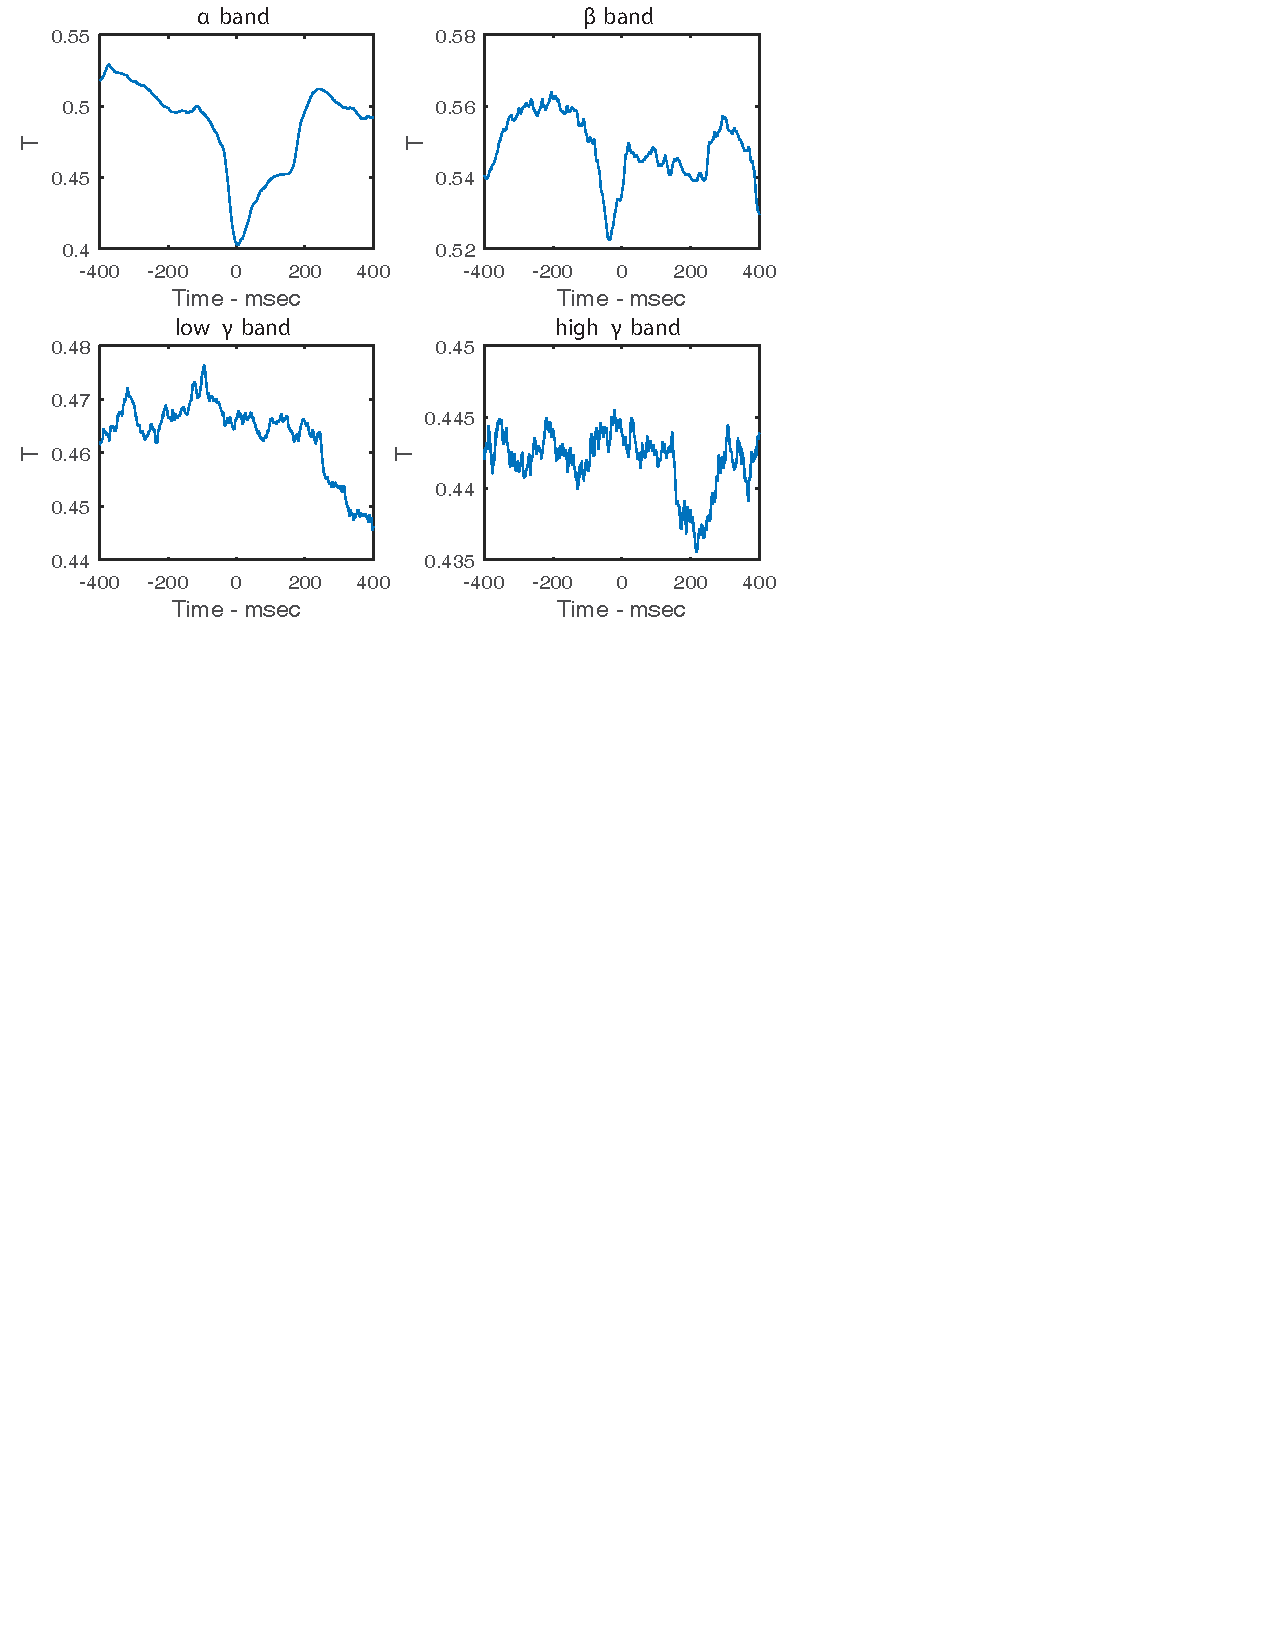
\includegraphics[scale=0.6]{T_Multiple_Bands.pdf}
                             \end{center}
                                                          \vspace{-4.2in}
                             \caption{\label{fig:GC_low} Network transitivity $T$ for the four bands of LFPs.}
\end{figure}


The mean average path lenghts $L$  for evoked responses across all channels for the four different frequency bands were shown in Fig. \ref{fig:GC_high}. Unlike the network transitivity measure $T$, the values of the average path length $L$ was inversely proportional to the frequency bands. For $L$, the $\alpha$ and $\beta$ bands were not sharing similar profiles in comparison to $T$. The $\alpha$ band exhibited a small variation until a local minima around $-100$ ms, then a sudden increase up to $0$ ms, then a decay. On the other hand, the $\beta$ band showed somewhat constant values of $L$ except for around $-200$ ms. The low $\gamma$ band did not show significant modulation in its spectrogram, but the path length showed a dynamical behavior where a sudden drop in $L$ took place around $-175$ to $-150$ ms followed by a monotonic increase. The high $\gamma$ showed a local maxima at around $-130$ ms followed by a decrease up to around $-15$ ms.
 
 
\begin{figure}[ht!]
                             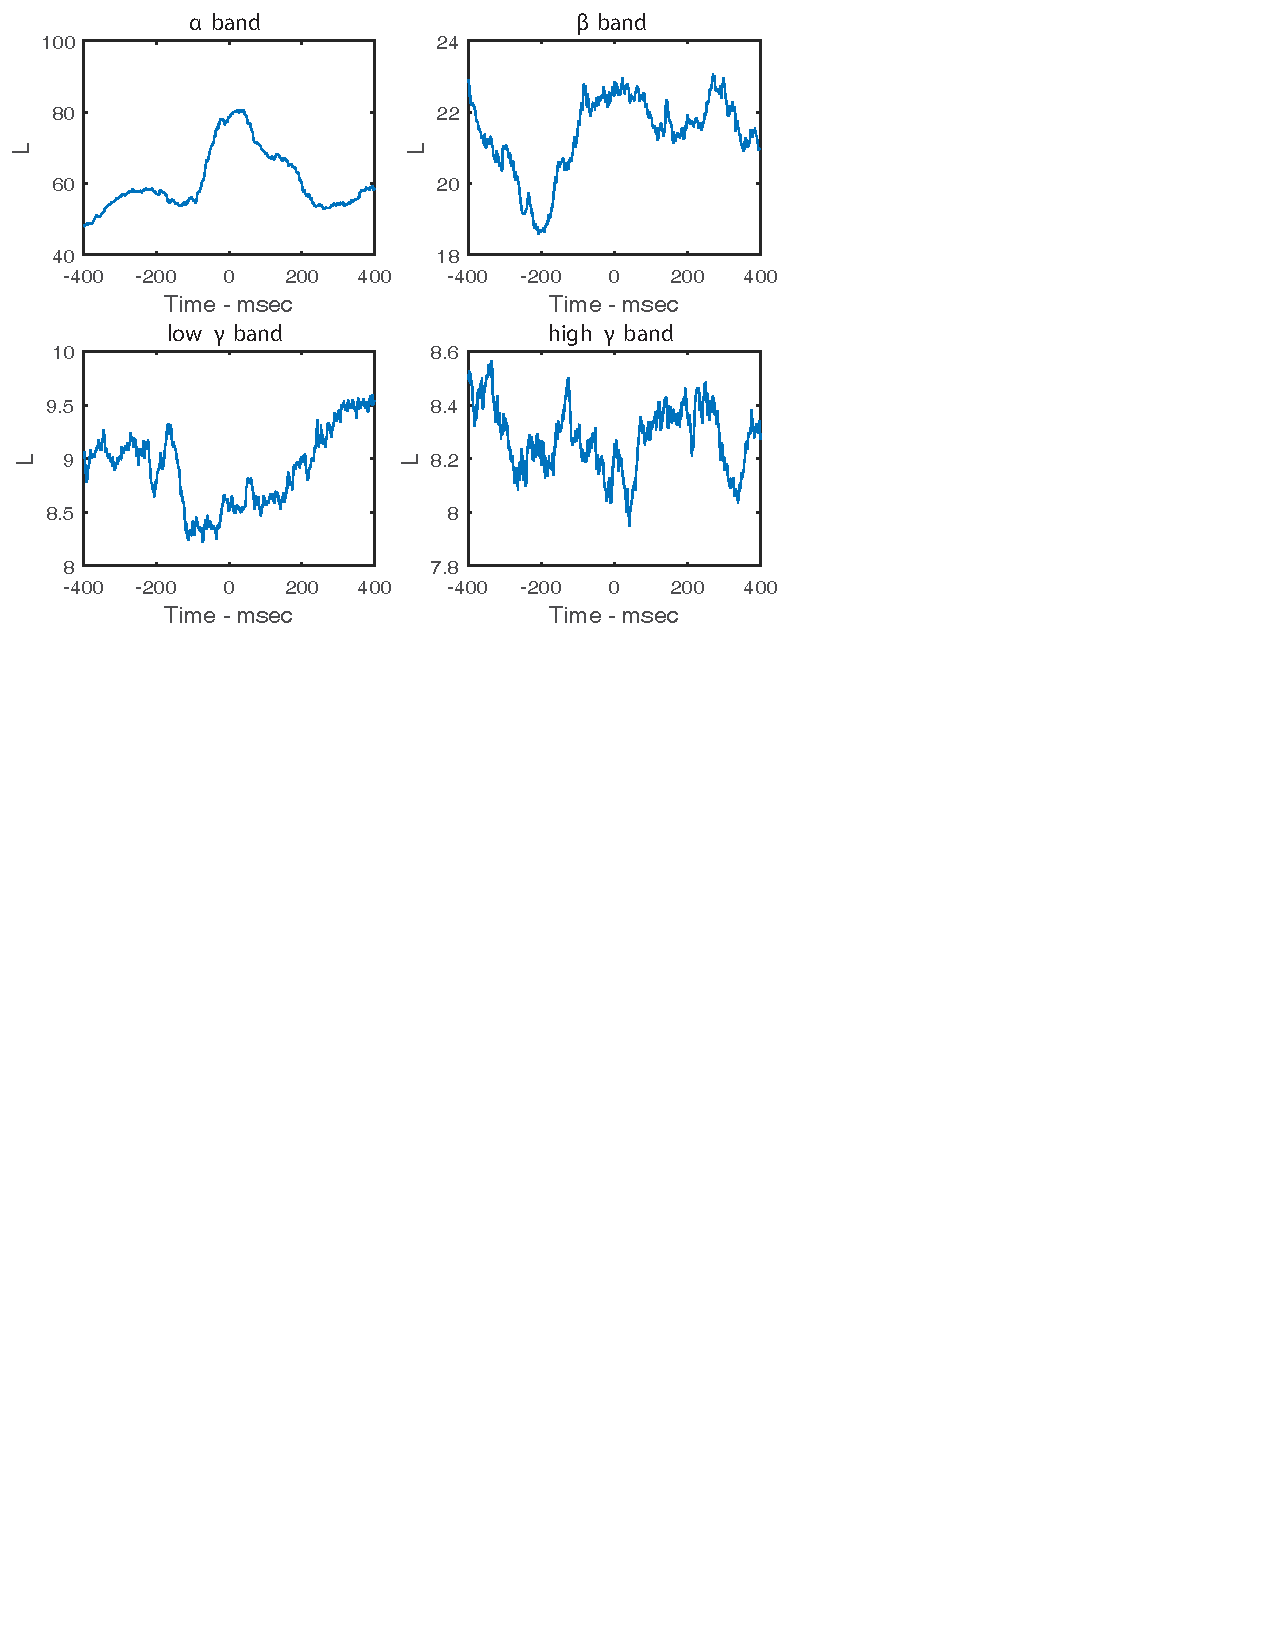
\includegraphics[scale=0.6]{L_Multiple_Bands.pdf}
                             \vspace{-4.2in}
                             \caption{\label{fig:GC_high} Average path length $L$ across the four bands of LFPs.}
\end{figure}

 
% \begin{figure}[ht!]
%                             \includegraphics[scale=0.35]{low_vs_high_C_variation.pdf}
%                             \caption{\label{fig:GC_comp} Variations of global clustering coefficients across channels for the two different bands. Each plot shows mean $\pm$ std computed over all the channels used for the analysis. Top for low frequency range, [1,30]Hz. Bottom for high frequency (or low $\gamma$ range [30,80]Hz. }
%\end{figure}

%
%  \subsection{Optimal delay}
%  
%  Fig. \ref{fig:OptDelay} shows the auto-mutual information for an exemplary channel. It can be seen from Fig. \ref{fig:OptDelay}  that the first local minimum of the auto-mutual information occurs at a lag of 5. Similar behavior was seen for most of signals from other channels. 
%%\begin{figure}[ht!]
%%                             \includegraphics[scale=0.5]{fig3.pdf}
%%                             \caption{\label{fig:OptDelay} Optimal delay $\tau$ using auto-mutual information for an exemplary channel. The red line denotes the first local minimum.}
%%\end{figure}
% 
% \subsection{Embedding dimension}
%
%Fig. \ref{fig:min_emb}  shown the plot of FNN statistic with respect to the embedding dimension for an exemplary signal. Already at an embedding dimension of 3, the value of FNN statistic drops to 0.04. Given the amount of data in each window (150 sample points), the choice of m = 3 seems feasible. Going for larger values of m like 5 or 6 might greatly reduce the amount of points needed to estimate the network characteristics. For the sake of consistency, based of these observations, we set optimal delay $\tau = 5$ and embedding dimension $m = 3$  to reconstruct the phase space vector from all the signals.

%\begin{figure}[ht!]
%                             \includegraphics[scale=0.5]{fig4.pdf}
%                             \caption{\label{fig:min_emb} Minimum embedding $m$ using the FNN method for an exemplary channel. At $m=3$, the FNN statistic is already below 0.05}
%\end{figure}


\section{Discussions}
\label{sec:discussions}
We characterized the evoked responses of intracortically recorded LFPs from MIo across the four bands $\alpha$, $\beta$, low $\gamma$, and high $\gamma$. The $\beta$ band showed some modulations in terms of its power profile against swallow cycle onsets, not EMG onsets as in \cite{Teismann2009}. Thus, our simple spectral analysis further suggests that the $\beta$ range in MIo is a band of interest to establish relation between swallowing and LFPs. Our new RN method shed a light to exhibit that potentially other bands could be related to swallowing behavior. The network transitivity, $T$, of the $\alpha$ and $\beta$ bands showed comparable temporal profiles, sharp drop of $T$ values start before $0$ ms, while the temporal evolution of power themselves have any similar relation. It is not clearly definitive, based on this preliminary study, that this sharp drop prior to $0$ ms in both $\alpha$ and $\beta$ is a signature of swallowing, however, this will be a hypothesis to be tested in our future study with data from more animals. 

Based on the analysis of average path length, $L$, the $\alpha$ and the $\beta$ bands show dissimilar temporal evolutions especially at the times of their local minima, $-175$ ms and $-200$ ms respectively. Thus, those reduction in $L$ on both bands may indicate a timing similar to what we commonly observe as ERD in $\beta$ oscillation around movement onset for visuomotor task with upper limb. Although swallowing is not a visuomotor behavior, the cortical $\beta$ activity decreases its periodic or synchronized oscillatory activities across the entire recording area from MIo. The behavioral relevance of this decrease is clearly unknown, but this may reflect a decison of a swallow reflected in the cortex. Furthremore, another set of local minima around $200$ ms and $150-200$ ms for those two bands is happening right around the time that actual swallowing activity takes place (data not shown). Thus a decrease in $L$ to reach to those local minima may indicate another type of an important event such as  kinematic coordination of tongue, jaw, and other oropharyngeal components involved in swallowing or change in cortical-subcortical interactions such that ``noisy'' cortical activity would not affect semi-automatic reflex movement, swallowing, controlled by the brainstem swallow center. 
Although these dynamical measures are not computable in real time, they guide us as to which time window we need to look at in relevant neural, kinematics, or kinetic signals. 

 In our current study, we only looked at evoked movements locked to swallow cycle onsets across all channels. However, we are in the process to expand this analysis to single trials as well as to develop statistical assessment of peaks in various network measures not limited to $T$ and $L$ used in this study. Furthermore, the variability of those network measures in different channels has to be studied. Our array spans $4$x$4$ mm in the orofacial cortex, but as it has been shown \cite{Hatanaka2005} that local responses characterized by intracortical microstimulation (ICMS) are fairly heterogeneous. Therefore, we need to incorporate either functional or spatial interactions of these measures from all the channels from our arrays to further advance our understanding of cortical LFP dynamics and its relation to swallowing or other orofacial behaviors. 




\section{Acknowledgement}
The authors would like to thank  members of Hatsopoulos laboratory at University of Chicago for surgery,  training, and data collection from monkeys and discussions. This work was completed in part with resources provided by the University of Chicago Research Computing Center (RCC).

\bibliographystyle{IEEEbib}
\bibliography{refs}
\end{document}